\documentclass[12pt]{report}
\usepackage{graphicx}
\graphicspath{ {images/} }
\begin{document}
  \section{What a genetic algorithm is}
  \subsection{Theory}
  \section{Advantages of genetic algorithms}
  \section{genetic algorithms for timetabling problems}
  \subsection{Choosing the right algorithm}
  \subsubsection{Why use uniform crossover as our recombination operator?}
  In most real world university timetabling problems, students are not uniformly
  distributed between modules. Instead, students tend to take related modules
  and there are therefore relatively few clashes between dissimilar modules such
  as between an archeology module and a mathematics module. This means that the
  bulk of constraints exist within relatively small subsets of the set of
  events. If we consider one such subset, the existence of many constraints
  between the members of this subset means that there will be few compatible
  assignements for members of this subset. A usefull building block might
  therefore be given by any such coherent assignement.\cite{Fang}
  A good recombination operator would therefore seek to preserve such building
  blocks. However, if we do not know in advance what the highly constrained
  subsets of events are, the building blocks may have long defining length, and
  would therefore be disrupted by a N-point crossover. However this isn't the
  case with a uniform Crossover.
  \subsection{Why the Wednesday tutorial timetabling problem is different}
  In a normal University timetabling problem, students attend a certain set of
  events, and the problem is to schedule these events so that there are no
  clashes. At a university level, a very large number of events can be scheduled
  into a much smaller amount of timeslots (around 40-50 a week) because most
  events don't have any students in common. Furthermore, all students attending
  a certain event (a lecture for example), actually attend the same concrete
  lecture bar certain exeptions (ie: there are not two different sets of Galois
  Theory lectures going on for different groups of students.) In this regards, the Wednesday
  morning tutorial problem is very different. Firstly, as the following heatmap
  shows, every pair of Mathematics modules of a given level has at least 50
  students in common. Therefore if we were to try and schedule events such as
  MTH1001tutorial the trivial solution of scheduling one event per
  timeslot is also the optimal one. This means that, in order to fit students
  into less timeslots than 4, we cannot only start splitting students into
  groups once timeslots are assigned.
  \begin{figure}
    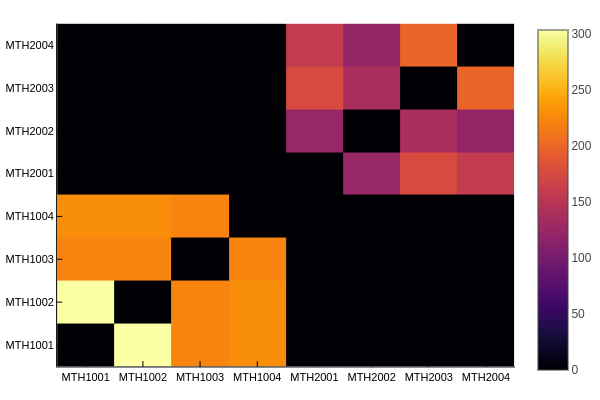
\includegraphics[width=100mm]{module-clashes}
  \end{figure}
\end{document}